\documentclass{standalone}
\usepackage{tikz}
\usepackage{ctex,siunitx}
\setCJKmainfont{Noto Serif CJK SC}
\usepackage{tkz-euclide}
\usepackage{amsmath}
\usetikzlibrary{patterns, calc}
\usetikzlibrary {decorations.pathmorphing, decorations.pathreplacing, decorations.shapes,}

\begin{document}
\small
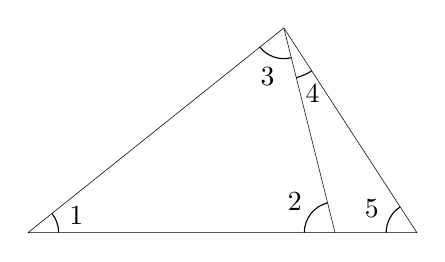
\begin{tikzpicture}[>=stealth,scale=1.3]
  \tkzSetUpPoint[fill=black]
  % \useasboundingbox(-1,-0.75)rectangle(3.7,1.4);
  \tkzDefPoints{0/0/A, 3/0/B, 3.8/0/C, 2.5/2/D}
  \tkzDrawPolygon(A,C,D)
  \tkzDrawSegments(B,D)
  \tkzMarkAngles[mark=none, size=.3](C,A,D D,B,A A,D,B D,C,A)
  \tkzLabelAngle[pos=.5](C,A,D){1}
  \tkzLabelAngle[pos=.5](D,B,A){2}
  \tkzLabelAngle[pos=.5](A,D,B){3}
  \tkzLabelAngle[pos=.5](D,C,A){5}
  \tkzMarkAngles[mark=none, size=.5](B,D,C)
  \tkzLabelAngle[pos=.7](B,D,C){4}
\end{tikzpicture}
\end{document}